\documentclass{article}
\usepackage[fleqn]{amsmath}
\usepackage{amssymb,graphicx,color,graphicx,slashed, microtype, parskip, enumitem, extarrows, needspace}
%\usepackage[utf8x]{inputenc}
\usepackage[top=1.5cm, bottom=1.5cm, right=6cm, left=1.5cm, heightrounded, marginparwidth=5cm, marginparsep=0.5cm]{geometry}

\hbadness = 10000
\hfuzz=100pt 
    
\usepackage{marginnote}
\renewcommand*{\marginfont}{\footnotesize}

\usepackage{hyperref}
\hypersetup{colorlinks=true, urlcolor=NavyBlue, bookmarksdepth=3}

\makeatletter\newcommand{\@minipagerestore}{\setlength{\parskip}{\medskipamount}}\makeatother

% =============== Index ===========================

\usepackage[nonewpage]{imakeidx}
\makeindex

% =============== Color Definitions ===============
    
\usepackage[svgnames]{xcolor}
\colorlet{ColorTitle}{Black}
\colorlet{ColorSectionName}{Black}
\colorlet{ColorBoxFG}{Gray}
\colorlet{ColorBoxText}{Black}
\colorlet{ColorBoxBG}{White}


% =============== Title Style ===============
    
\usepackage{titling} % Allows custom title configuration
    
\newcommand{\HorRule}{\color{ColorTitle}\rule{\linewidth}{1pt}} % Defines the gold horizontal rule around the title
    
\pretitle{
    \vspace{-50pt} % Move the entire title section up
    \HorRule\vspace{9pt} % Horizontal rule before the title
    \fontsize{27}{36}\usefont{OT1}{phv}{b}{n}\selectfont
    \color{ColorTitle} % Text colour for the title and author(s)
}
    
\posttitle{\par\vskip 15pt} % Whitespace under the title
    
\preauthor{\fontsize{17}{0}\usefont{OT1}{phv}{m}{n}\selectfont\color{ColorTitle}} % Anything that will appear before \author is printed
    
\postauthor{\par\HorRule}

\newcommand{\COURSENAME}{\href{http://phyw.people.ust.hk/teaching/PHYS2022-2015/}{\textcolor{black}{PHYS 2022}}}
\newcommand{\YW}{\href{http://phyw.people.ust.hk/}{\textcolor{black}{Yi Wang}}}
\newcommand{\PHYS}{\href{http://physics.ust.hk}{\textcolor{black}{Department of Physics}}}
\newcommand{\HKUST}{\href{http://www.ust.hk/}{\textcolor{black}{HKUST}}}
\author{\COURSENAME, \YW, \PHYS, \HKUST}

\date{}

% =============== Section Name Style ===============
    
\usepackage{titlesec}
    
\titleformat{\section}
    {\fontsize{15}{20}\usefont{OT1}{phv}{b}{n}\color{ColorSectionName}}
    {\thesection}{1em}{}
    %[{\vspace{0.2cm}\titlerule[0.8pt]}]
    
\titleformat{\subsection}
    {\fontsize{14}{20}\usefont{OT1}{phv}{m}{n}\color{ColorSectionName}}
    {\thesubsection}{1em}{}
    
\titleformat{\subsubsection}
    {\fontsize{12}{20}\usefont{OT1}{phv}{m}{n}\color{ColorSectionName}}
    {}{0em}{}
      
\setcounter{secnumdepth}{4}
        
% =============== Box Style ===============
    
\usepackage[most]{tcolorbox}
    
\newtcolorbox{tbox}[1]{
    colback=ColorBoxBG, colframe=ColorBoxFG, coltext=ColorBoxText,
    sharp corners, enhanced, breakable, parbox=false,
    before skip=1em, after skip=1em,
    title={#1}, fonttitle=\usefont{OT1}{phv}{b}{n}, 
    attach boxed title to top left={yshift=-0.1mm}, boxed title style={sharp corners, colback=ColorBoxFG, left=0.405cm},
    rightrule=-1pt,toprule=-1pt, bottomrule=-1pt
}

\newtcolorbox{mtbox}[1]{
    colback=ColorBoxBG, colframe=ColorBoxFG, coltext=ColorBoxText,
    sharp corners, enhanced, breakable, parbox=false,
    before skip=1em, after skip=1em,
    title={#1}, fonttitle=\usefont{OT1}{phv}{b}{n},
    attach boxed title to top left={yshift=-0.1mm}, boxed title style={sharp corners, colback=ColorBoxFG, left=0.15cm},
    rightrule=-1pt,toprule=-1pt, bottomrule=-1pt, 
    left=0.5em
}

% =============== tikz has to be loaded after xcolor
\usepackage{tikz}

\newcommand*\enumlabel[1]{\tikz[baseline=(char.base)]{
			\node[shape=rectangle,inner sep=2pt,fill=ColorBoxFG] (char) 
			{\fontsize{7}{20}\usefont{OT1}{phv}{b}{n}{\textcolor{ColorBoxBG}{#1}}};}}

% =============== Useful shortcuts ===============

\newcommand\wref[1]{{\hypersetup{linkcolor=white}\ref{#1}}}  

\newcommand{\textbox}[2]{
    \begin{tbox}{#1}
        #2
    \end{tbox}
}

\newcommand{\mtextbox}[2]{\marginnote{
    \begin{mtbox}{#1}
        #2
    \end{mtbox}}
}

\newcommand{\mnewline}{\vspace{0.5em}\newline}

\newcommand{\titem}[1]{
    \begin{itemize}[label=\color{ColorBoxFG}$\blacktriangleright$, leftmargin=0mm, labelsep=0.27cm, topsep=0.5em
        %, itemsep=1ex
        ]
        #1
    \end{itemize}
}

\newcommand{\mtitem}[1]{
    \begin{itemize}[label={\color{ColorBoxFG}$\blacktriangleright$}, leftmargin=0mm, labelsep=1mm, topsep=0.5em
        %, itemsep=1ex
        ]
        #1
    \end{itemize}
}

\newcommand{\itembox}[3]{
    \begin{tbox}{#1}
        #2
        \titem{#3}
    \end{tbox}
}

\newcommand{\mitembox}[3]{
    \marginnote{
    \begin{mtbox}{#1}
        #2
        \mtitem{#3}
	\end{mtbox}
    }
}

\newcommand{\tenum}[1]{
    \begin{enumerate}[label=\protect\enumlabel{\arabic*}, leftmargin=0mm, labelsep=0.265cm, topsep=0.5em
        %, itemsep=1ex
        ]
        #1
    \end{enumerate}
}

\newcommand{\enumbox}[3]{
    \begin{tbox}{#1}
        #2
        \tenum{#3}
    \end{tbox}
}

\newcommand{\twocol}[5]{
    \begin{minipage}[t][][b]
        {#1\textwidth}
        #4        
    \end{minipage}
    \hspace{#2\textwidth}
    \begin{minipage}[t][][b]
        {#3\textwidth}
        #5
    \end{minipage}
}

\newcommand{\cg}[2]{
    \begin{center}
        \includegraphics[width=#1\textwidth]{#2}
    \end{center}
}

\newcommand{\tbar}{
    ~\newline
    {\color{ColorBoxFG}
    \hbox to 0.15\textwidth{\leaders\hbox to 5pt{\hss  \hss}\hfil} 
    \hbox to 0.7\textwidth{\leaders\hbox to 5pt{\hss . \hss}\hfil}}
    \mnewline
}

% =============== Filter unwanted warnings
\usepackage{silence}
\WarningsOff[tcolorbox]
\hbadness=1000000


\graphicspath{{7_fig/}}
\usepackage{ctex}
\title{第七章\ 从作用量到自然法则}

\begin{document}

\maketitle

\mtextbox{运动方程}{
    用来推算粒子运动路径的一个关于时间的二次微分方程(或方程组)叫做运动方程。\index{运动方程}比如说,粒子在势 $V(q)$ 中的运动可以用运动方程$\ddot q + dV/dq = 0$来描述。解实际问题的时候,运动方程还包含了初始条件:初始时间$t_0$以及$q(t_0)$与$\dot q(t_0)$的值。求解具有这种初始条件的运动方程称为柯西问题。\index{柯西问题}.
}
\textbox{一种新的物理思维方式}{
    我们习惯用牛顿的方式思考物理--对于粒子来说,如果我们知道初始位置和速率,我们可以计算该粒子一段时间的路径。这种思维方式可以推广到重力、电磁场、及其他概念上。

    但是如果我们真的想要思考基础的问题--这些运动方程能否成为自然的终极密码——仍然有一些不完美的方面:
    
     \tenum{
        \item 运动方程在狭义相对论中不是不变的对象,因为运动方程是时间演化的。在相对论中,时间和空间有几乎相同的权力。对于不同的观测者,运动方程是(以洛伦兹变换)协变,而非不变。自然的终极密码真的那么主观吗?在电影黑客帝国中,整个世界都是一个程序。那些程序员是否在这部电影中只选择了一个喜欢的帧来写下运动方程并对世界进行编码?
        \item 那些守恒定律是从哪里来的?我们知道能量、动量、角动量、电荷守恒定律。在特定的理论框架下,我们可以证明它们。比如说,在牛顿力学的框架下,我们可以运用聪明的技巧来证明能量和动量守恒。但是是否存在一个通用方法来找出所有系统的守恒定律的起源?
        \item 受限运动。比如说,想象一个钟摆(如果太简单,想象两个)。
        理想理论下,受限运动意味着我们减少了运动的可能性,从而使情况更简单。但是在牛顿物理中,越多限制意味着越多力的分析与更复杂的数学。有没有一种方法可以让受限系统更方便计算呢?
        \item 量子世界与与之对应的经典世界有很大的不同。我们还没有介绍量子力学,但是之后我们会解决这个问题。
        \item 这些运动方程对于解释自然的“习性”来说太“冷血”了。你可以用一句话概括自然法则(适用于所有已知基础物理)吗?比如说,“自然一般会$\cdots$”?仅仅说自然一般会满足运动方程似乎不足够信服别人。 
    }
    \tcblower
    莫佩尔蒂(1698-1759)说的一个短句很好地解决了以上问题:

    “自然的一切行为都是最简洁的。” \index{最小作用量原理}

    我们将看到这个简单的句子是如何工作的。
}

\section{费马原理}\label{sec:fermat}

在解决最小作用量原理之前,我们先用费马原理\index{费马原理}来研究光的传播。这还不是真正的最小作用量原理,但是它的物理概念和数学方法是极其相似的。它也是非常直观的,所以我们先做一个热身练习。

\mtextbox{皮埃尔·德·费马}{
    皮埃尔·德·费马(1601或1607 - 1665)是一个法国律师。不过没人记得他为什么案子辩护过。我们只记得他的一些其他事情,例如他对于$n>2$,$x^n+y^n=z^n$ 没有正整数解的猜想。直到300年后,这个猜想才在1994年被证明。
}
\textbox{费马原理}{
    \twocol{0.3}{0.05}{0.65}{
        考虑一类光传播的问题:已知两个定点$P$和$Q$,光是如何在两点之间传播的?
    
    右图给了可用空间的传播、反射、折射的例子。
    }{
        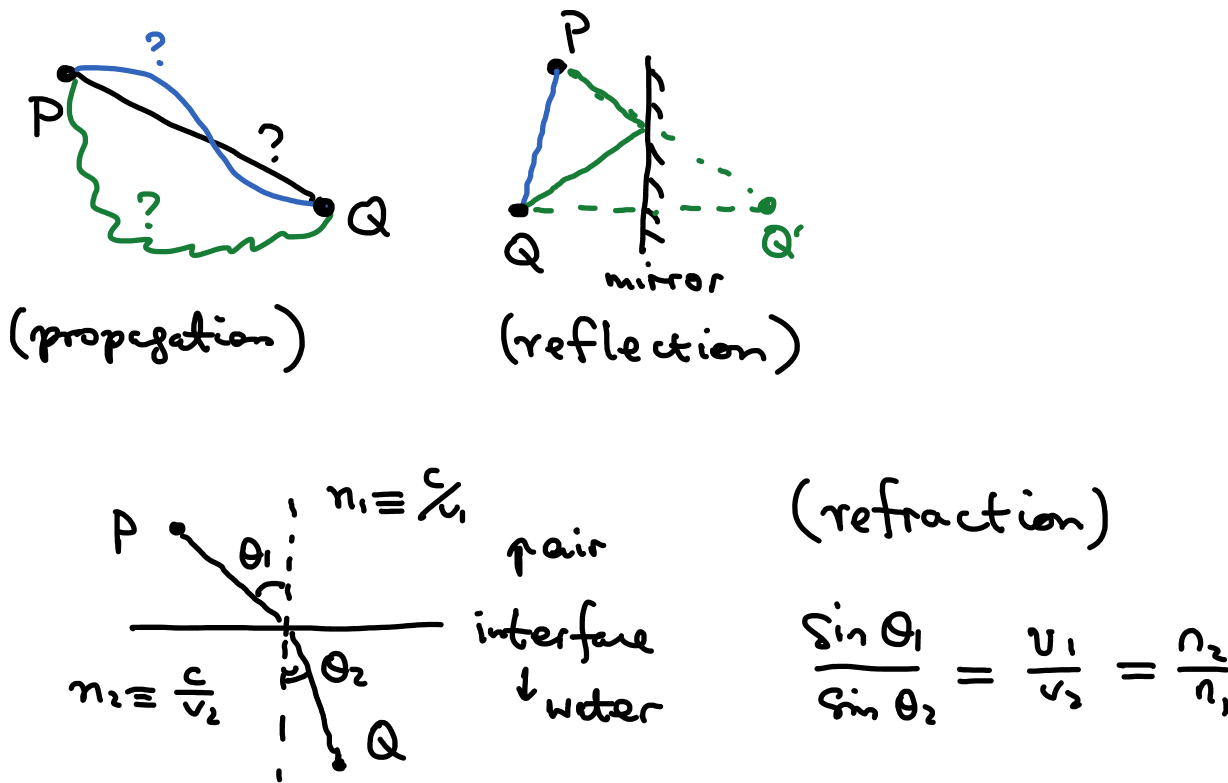
\includegraphics[width=\textwidth]{fermat}   
    }

    \tcblower

    费马提出了一个对这种问题的通用答案:光沿着极值时间的路径在两个已知点之间传播。
}

\textbox{行动时间如何取决于路径?泛函}{
    我们在微积分中熟知了极限问题:一个函数$f(x)$在$df/dx=0$时取极限值。我们这里的情况很相似,只不过使用不同的数学对象..

    \marginnote{当然并不是所有路径都可以被$y=y(x)$参数化,比如说x为常数。这里我们只关注可以被$y=y(x)$参数化的路径,因为它们可以提供足够的背景来推导最小作用量原理。}
    我们说的是空间(数学意义)的“路径”。怎么在数学中参数化一个路径呢?一个路径可以被看成一个函数。比如说,一个曲线$y=y(x)$。

    假设我们知道光速(真空中为$c$,在折射率$n$ 的介质中为$c/n$)。已知一个路径,我们可得光的传播时间$T$。这里的$T$取决于整个函数$y$(而不是$y(x)$在不同$x$时候的值)。我们可以说$T$是一个$y$的\emph{泛函},写做$T[y]$。
    
    长话短说,泛函是一个“函数的函数”。\index{泛函} 下图显示了函数和泛函的对比。

    \mtextbox{函数式编程}{在编程语言中,有个典范叫函数编程。它最基本的要求是你可以将函数作为另一个函数的参数传递。它与泛函一样(都是函数的函数)。}

    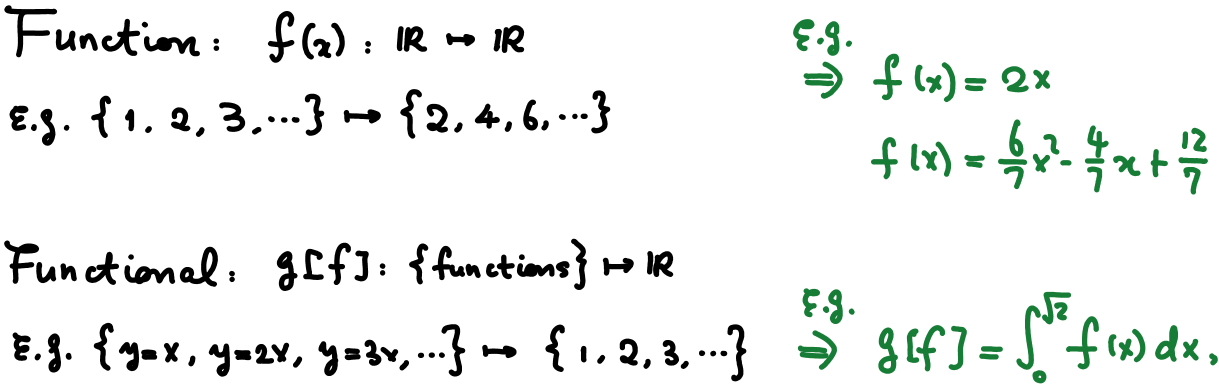
\includegraphics[width=0.8\textwidth]{functional}
}

\needspace{0.15\textheight}
\marginnote{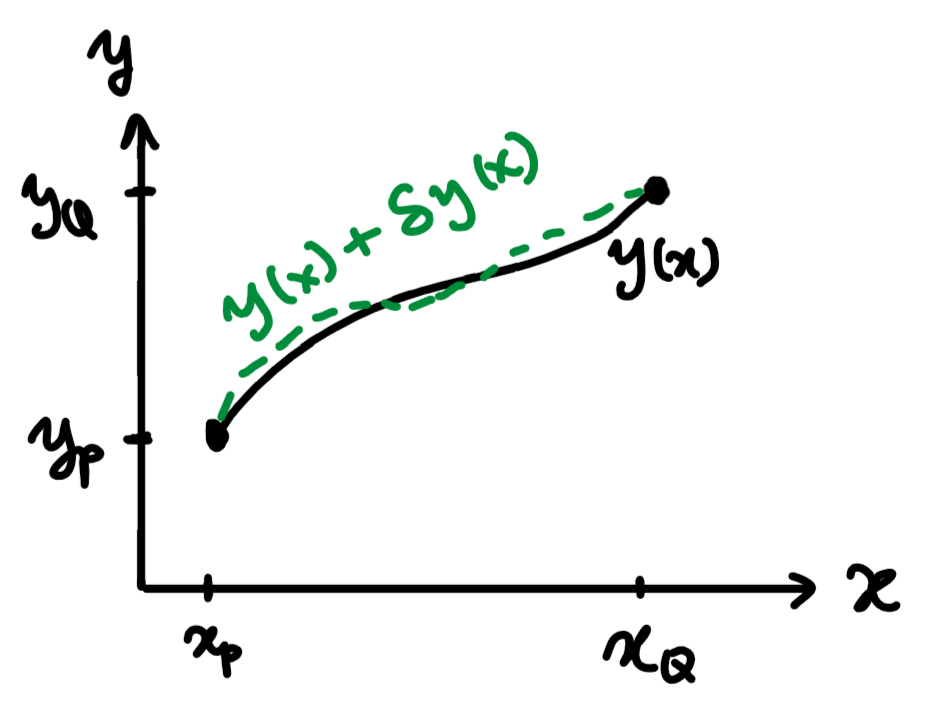
\includegraphics[width=0.3\textwidth]{variationyx}}
\textbox{哪个路径有极限时间?变分法\index{变分法}}{
    为了求$(x_P, y_P)$与$(x_Q, y_Q)$的极限时间,我们先画一个(通用)满足$y(x_P)=y_P$和$y(x_Q)=y_Q$的路径$y(x)$。然后我们找一些极限路径必须满足的条件。运用以下步骤:
    
    我们通过$y(x) \rightarrow y(x)+\delta y(x)$改变路径。$\delta y$为\emph{任意}无穷小函数(即我们可以忽略$(\delta y)^2$) 且满足$\delta y(x_P)=0$和$\delta y(x_Q)=0$。这些“边界条件”需要被满足,因为根据问题的定义,我们已经确定了这两个边界点。

    那么现在新路径的时间为$T[y+\delta y]$,泛函为
    \begin{align}
        \delta T \equiv T[y+\delta y] - T[y]~.
    \end{align}
    \mtextbox{为什么$\delta T=0$代表了极值?}{原因与在微积分里为什么函数$y(x)$在 $dy/dx=0$的时候有极值很相似。假设这个极值是一个局部最小值。考虑$y(x)$在$(x, x+dx)$之间的变化,保持在这个区域外的固定(这是 $\delta y$一种允许的形式)。那么如果$\delta T\neq 0$在$(x, x+dx)$之间,变化$\delta T = (\cdots) \delta y dx$。如果$(\cdots)$是负数,变化$\delta y$让$T$更小。那么$T$就不是最小值。如果$(\cdots)$是正数,那么变化$-\delta y$让$T$更小。那么$T$仍然不是最小值。因此,对于最小的 $T$,$\delta T$ 在 $(x, x+dx)$ 内消失。由于 $(x, x+dx)$ 是一个区间,$\delta T$ 应该在任何地方都消失。 局部最大值的证明同理。}
    对于所有可能的变化$\delta y(x)$,极值时间的路径一定满足$\delta T = 0$。
}

以上可能看着很枯燥和空洞。那么我们来看一个例子。

\textbox{真空中光的传播}{
    我们研究的光在$(x_P, y_P)$与$(x_Q, y_Q)$之间自由传播。假设我们只知道费马定理和光速为$c$。为了简单来说,我们抑制了$z$方向。我们只研究$x,y$空间维度。两点之间的传播时间$T$可以写为
    \begin{align}
        T = \int_{t_P}^{t_Q} dt 
        = \frac{1}{c} \int_{x=x_P, y=y_P}^{x=x_Q, y=y_Q} \sqrt{dx^2 + dy^2}
        = 
        \frac{1}{c} \int_{x_P}^{x_Q} \sqrt{1 + \left(\frac{dy}{dx}\right)^2 } ~ dx ~.    
    \end{align}
    为了找到极限路径$y(x)$必须满足的条件,我们改变 $y(x)\rightarrow y(x)+\delta y(x)$并带入以上等式。因为 $d\delta y / dx$非常小,我们可以当它是一个极小参数并进行泰勒展开:
    \begin{align}
        \label{eq:integrand}
        \sqrt{1 + \left(\frac{d[y(x)+\delta y(x)]}{dx}\right)^2 }
        = \sqrt{1+(y')^2} + 
        \frac{y'}{\sqrt{1+(y')^2}} \frac{d \delta y}{dx} + \mathcal{O}[(\delta y)^2]~, 
      \end{align}
      这里$y'\equiv dy(x)/dx$。因此
      \begin{align}
        \label{eq:Tvariation}
        \delta T[y] & = \frac{1}{c} \int_{x_P}^{x_Q}
        \frac{y'}{\sqrt{1+(y')^2}} \frac{d \delta y}{dx} ~ dx \nonumber\\ &
        = \frac{1}{c} \int_{x_P}^{x_Q} \left\{
        \frac{d}{dx} \left ( \frac{y'}{\sqrt{1+(y')^2}} \delta y \right ) 
        - \delta y \frac{d}{dx} \left ( \frac{y'}{\sqrt{1+(y')^2}} \right ) \right\} 
        ~ dx \nonumber\\ &
        = - \frac{1}{c} \int_{x_P}^{x_Q} 
        \delta y \frac{d}{dx} \left ( \frac{y'}{\sqrt{1+(y')^2}} \right )  
        ~ dx~,
      \end{align}  
      这里我们完全忽略了导数项因为$\delta y=0$在边界上。

      $\delta T=0$需要使以上等式对于所有$\delta y$都消失。因此我们需要满足
      \begin{align}
        \label{eq:yvariation}
        \frac{d}{dx} \left ( \frac{y'}{\sqrt{1+(y')^2}} \right) = 0
        \quad\rightarrow\quad
        y'=\mbox{const}~.
      \end{align}
      我们就证明了费马定理中的光沿直线运动。
}

通过更多的努力,我们可以通过费马定理及一些变形式推算出反射、折射的光的路径。但是这里我们不会做。

这里我们是在运用很复杂的方法来做一个很简单的事情。但是这里提出的技术(数学)会在关于运动定理的下节被重新运用。

\section{极值作用原理}

人可以用两种方法来过一生:(一)已知现在的状态,我满足于现在的状态。我会与时俱进来看看未来会怎么样;(二)已知现在的状态,我有一个对未来的清晰的梦想。我会对未来有个总体规划从而让梦想成真。

有趣的是,物理也可以被跟这两种等同的方式被理解:(一)与柯西问题相对应 -- 用初始位置及速率来求运动方程;(二)与作用原理相对应,我们接下来就来介绍它。

\textbox{作用原理\index{作用原理}}{
    理论由行动$S$定义。这个理论的运动方程与极限运动$\delta S = 0$相对应。
}

让我们先看看这个在牛顿力学中是怎么应用的。之后我们会概括它到所有已知基础理论。

\marginnote{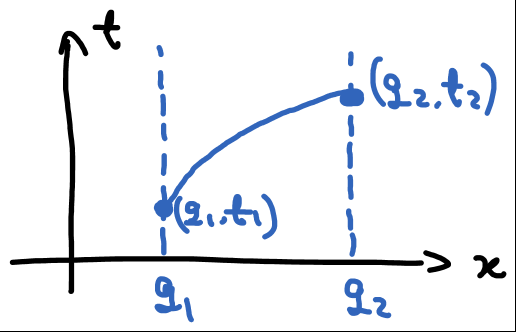
\includegraphics[width=0.3\textwidth, trim={0 2pt 2pt 0}, clip]{newton}}
\textbox{牛顿力学的作用原理}{\index{牛顿力学的运动}
    牛顿力学可以被以下问题制定:

    已知势$V(q)$,粒子从初始点$(q_1, t_1)$到终点$(q_2, t_2)$的行动路径是什么?($q(t)$为粒子的位置)

    首先我们先定义一个作用
    \mtextbox{关于积分的表达}{物理学家有时会写$\int dt f(t)$。这与$\int f(t) dt$一样,只是写法的不同而已。但是这也反映了物理学家一般会把积分想成和的极限:$\lim_{\Delta t\rightarrow 0} \sum_i \Delta t f(t_i) = \int dt f(t)$。这里的$\Delta t$和 $f(t_i)$只是被乘在一起,所以顺序就不重要了。}
    \begin{align}
    \label{eq:newtonAction}
    S[q] = \int_{t_1}^{t_2} dt \left [ 
    \frac{1}{2} m \dot q ^2 - V(q)
    \right ]~.
    \end{align} 
    这个作用的形式是$K-V$对于时间的积分,$K$为动能、$V$为势能。这个形式很笼统。现在不用对它的物理意义有疑问。我们仅仅定义了一个泛函(路径$q(t)$的泛函)来看它会带我们到哪儿。我们会回到它的物理意义(以及为何极限作用原理成立)在小节 \ref{sec:action-quantum}.

    如果要推导运动方程,与小节\ref{sec:fermat}类似,我们改变$q(t)\rightarrow q(t)+\delta q(t)$,从而满足$\delta q(t_1)=\delta q(t_2) = 0$。然后观察作用的变化:
    \mtextbox{被限制的运动}{现在,你应该已经可以求解被限制的运动了。比如说,运用比牛顿对力的分析更巧妙的方法来求解双摆锤。作为一个练习,你可能会用两个角度来参数化系统的$K$与$V$ 然后写$S=\int dt (K-V)$。变化原理会给你一个比力的计算更简单的答案。}
    \begin{align}
        \label{eq:dSNewton}
        \delta S = \int_{t_1}^{t_2} dt 
        \left [ m \dot q \delta \dot q - \frac{dV}{dq} \delta q   \right ]
        = \int_{t_1}^{t_2} dt 
        \left [ \frac{d}{dt}(m\dot q \delta q) - m\ddot q \delta q - \frac{dV}{dq}\delta q  \right ]~.
    \end{align} 
    这个第一项是一个会消失的边界项。后两项对于所有$\delta q(t)$都成立。因此我们重新推到了牛顿力学的运动方程:
    \begin{align}
        \label{eq:eomNewton}
        m\ddot q + \frac{dV}{dq} =0~.
    \end{align}
}

\needspace{0.15\textheight}
\mtextbox{拉格朗日方程背后的数学}{$L=L(q_i, \dot q_i, t)$在多元微积分的意义是:假设其余两个变量不变,我们可以”独立地“求出每一个变量的偏导数。比如说,求$\partial_t L \equiv \partial L / \partial t$的时候,我们假设$q_i$和$\dot q_i$是不变的。这与 
\newline$dL/dt$ $= \sum_i (\partial L / \partial q_i)(dq_i/dt)$ 
\newline$+ \sum_i (\partial L / \partial \dot q_i) (d\dot q_i/dt)$ $+ \partial L / \partial t$是不同的。}
\textbox{通用作用与欧拉-拉格朗日方程}{\index{欧拉-拉格朗日方程}
    一般来说,考虑一个“拉格朗日方程”\index{拉格朗日方程} $L=L(q_i, \dot q_i, t)$。$i=1, 2, \ldots, N$。这里的$q_i$代表了第$i$个粒子的位置。(事实上,在广义坐标里,指数$i$可以代表很多东西:不同的空间维度、不同的粒子、在某点的各个场的值…… 我们不会考虑这些细节。)
    
    作用被定义为
    \begin{align}
        \label{eq:actionL}
        S = \int L(q_i, \dot q_i, t) dt~.
    \end{align}
    这里我们还没有写下积分的区间。记住边界项会被消除掉。很显然这里的定义包括了我们前面研究的牛顿粒子的例子也更广义了。

    这个更通用系统的运动方程(又被称为欧拉-拉格朗日方程)可以被这个变形推导出来
    \mtextbox{消除边界项}{
        从现在开始我们会假设所有边界项$\int \partial_t(\cdots) dt$都可以被消除掉。原因是这项不会影响运动方程。对边界项的详细处理方式远远超出了我们的学习范围,但是去掉这项不会影响我们现在做的任何事情。
    }
    \begin{align}
    \label{eq:dSEL}
    \delta S & = \sum_i \int \left ( 
    \frac{\partial L}{\partial \dot q_i} \delta\dot q_i  
    + \frac{\partial L}{\partial q_i} \delta q_i 
    \right ) dt \nonumber\\ &
    = \sum_i \int \left [
        \frac{d}{dt} \left ( \frac{\partial L}{\partial\dot q_i} \delta q_i \right )
        -  \frac{d}{dt} \left ( \frac{\partial L}{\partial\dot q_i} \right)\delta q_i
        + \frac{\partial L}{\partial q_i} \delta q_i
    \right ] dt~.
    \end{align}
    因此欧拉-拉格朗日方程(对所有$i$都成立)可以被看成
    \begin{align}
    \label{eq:eomEL}
    \frac{d}{dt} \left ( \frac{\partial L}{\partial\dot q_i} \right)
    - \frac{\partial L}{\partial q_i} = 0 ~.
    \end{align}
}

\textbox{用一行概括所有已知的基础物理}{
    所有已知的物理都可以被写成作用\index{标准模型的作用}
        \begin{align}
          \label{eq:SMaction}
          S \sim \int d^4 x \sqrt{-g} \Big\{ 
          \frac{1}{16\pi G}  R 
          - \frac{1}{4} F^2 
          + i \bar\psi \slashed{D} \psi 
          + |D h|^2 - V(h) 
          + h \bar\psi \psi 
          \Big\}~.
        \end{align}
    这个作用包含了引力($g$)、电磁及他们的好伙伴(规范场$F$)、电子及他们的好伙伴(旋量场$\psi$)、质量的起源(希格斯场$h$)。这些场与一些规范对称性被称为粒子物理的标准模型。它描述了所有已知基础物理。
    我们不会在这里解释它(需要一门粒子物理或者量子场理论的课)。现在把它当成一个艺术品吧。
    }

\section{对称性与守恒定理}

在狭义相对论讲相对动量与能量的时候,我们讨论了为什么需要那些守恒定理:(一)物理上,它们允许我们忽略过程中间的细节;(二)数学上,它们允许我们把二次常微分方程降到一次或者零次;(三)为现代物理学提供可观测量。

那么剩下的问题就是为什么守恒定理存在呢?如果要回答这个问题,我们应该用一个物理理论的通用框架来寻找守恒定理的根源。因此通用作用\eqref{eq:actionL}是一个很好的起点。

与其直接提问为什么\eqref{eq:actionL}中的东西都是守恒的,让我们先考虑这个等式的对称性的美。

\needspace{0.2\textheight}
\mtextbox{备注:对称性}{
    \mtitem{
        \item 作用是推导运动方程的一种方式。因此在检查\eqref{eq:sym-trans-q}中作用的变化时,任何运动方程都不应该用(避免循环论证)。更详细地说,在讨论$\delta S=0$的时候,我们是在说以下两件事中的一个:(一)不使用运动方程的对称变化;(二)任何变换(可能不是对称)作为变分原理,并使用运动方程。我们应该清楚它们之间的区别是什么。
        \item 这里我们仍然会在考虑作用的变化时消掉边界项$\int \partial_t (\cdots) dt$。也就是说如果拉格朗日量$L(\tilde q_i, \dot {\tilde q}_i, t) \neq L(q_i, \dot q_i, t)$,而是$L(\tilde q_i, \dot {\tilde q}_i, t) = L(q_i, \dot q_i, t) - \epsilon dg/dt$($g$为随机数)。这个变形也是对称的。
        \item 因为$\epsilon$是无穷小的,我们可以忽略$\mathcal{O}(\epsilon^2)$项。
        \item 我们学过的这种变形\eqref{eq:sym-trans-q}是连续与全局对称的。还存在有一些其他的对称性,类如离散对称与规范对称,但是它们对推导不简单的守恒定理是没用的。
    }
}
\textbox{理论的对称性}{\index{对称性}
    理论的对称性是理论在其下不会改变的变换。
    \tcblower
    按照\eqref{eq:actionL},以上对称性的定义可以更详细地说是:
    
    考虑一个无穷小的变换\index{变换}
    \begin{align}
        \label{eq:sym-trans-q}
        q_i \rightarrow \tilde q_i = q_i + \epsilon \delta q_i~,
    \end{align}
    $\epsilon$为一个无穷小的常数。如果作用量是不变的,
    \begin{align}
        \label{eq:sim-trans-s}
        \delta S = \int L(\tilde q_i, \dot {\tilde q}_i, t) dt - \int L(q_i, \dot q_i, t) dt = 0 ~,
    \end{align}
    那么变换\eqref{eq:sym-trans-q}是对称的。
}
\eqref{eq:sym-trans-q}和\eqref{eq:sim-trans-s}的定义是非常抽象的。因此让我们考虑以下的例子:
\textbox{变换的例子}{
    \titem{
        \item 时间平移\index{时间平移}来测试一个理论的预测是不是与时间相关的。这个变换关联了两种情况:现在做实验与等会再做实验(用同一理论),然后再看两个的区别。因此时间平移可以被写成
        \begin{align}
            q_i (t) \rightarrow \tilde q_i(t) = q_i (t + \epsilon \delta t) 
            = q_i (t) + \epsilon \dot q_i(t) \delta t~.
        \end{align}
        我们可以从中得出
        \begin{align}
            \delta q_i = \dot q_i(t) \delta t~.
        \end{align}
        我们会在此章中更深度地研究时间平移。
        
        \marginnote{在空间平移中,对于不同的$i$,$\delta q_i$是不是一致的?我们需要想$i$真正代表了什么:如果$i$代表了空间中不同的方向,那么可以是不同的值。如果$i$代表了同方向的不同粒子,那么对于不同的$i$,$\delta q_i$必须是同一个值。 }
        \item 空间平移,来测试同一个实验在不同地方做会不会有不同。这个变换是$q_i(t) \rightarrow q_i (t) + \epsilon \delta q_i$,$q_i$为常数偏移。空间平移与动量守恒有关。

        \item 洛伦兹变换。对于无穷小的$\beta$(或者旋转),$(t_B, x_B)$与$(t_A, x_A)$之间的升压。当$\beta$很小,$\gamma\approx 1$。然后大约$t_B \simeq t_A + \epsilon v x_A/c^2$、$x_B \simeq x_A + \epsilon v t_A$。我们可得$q_i(t) \rightarrow q_i (t+ \epsilon v q_i /c^2) + \epsilon v t$这个升压部分与(不是很有意思的)原能量中心有关。洛伦兹转换的旋转部分可以被差不多地定义。它与角动量守恒有关。

        \item 相变。如果$q_i$是复数,我们可以去考虑变换$q_i \rightarrow e^{i \epsilon \alpha} q_i$。这与电荷守恒有关。
    }
}

我们已经学过很多种变换了。那么让我们来探索一下一个对称转换的前提条件吧。我们会以时间平移为例子。
\textbox{什么时候时间平移是具有对称性的?}{
    \marginnote{注意$L=L(q_i, \dot q_i)$是时间平移对称性的充分条件但非必要条件。我们不会在这里探索这个必要条件。}
    如果由拉格朗日量$L$指定的理论并不明确由$t$而定(i.e. $L(q_i, \dot q_i,t)=L(q_i, \dot q_i)$,没有明确$t$的依赖性)那么很显然这个理论是时间平移不变量。这里我们会测试在这种情况下,时间平移是不是具有对称性。
    \tcblower
    时间平移下,如果$\epsilon$为常数,我们可以得到    \begin{align}
        \delta q_i = \dot q_i \delta t~, \qquad \delta \dot q_i = \ddot q_i \delta t~.
    \end{align}
    \begin{align}\label{eq:dL-time-translation}
        \delta L = L(q_i + \epsilon \dot q_i \delta t, \dot q_i + \epsilon \ddot q_i \delta t) 
        - L(q_i, \dot q_i)
        = \left [
            \frac{\partial L}{\partial q_i} \dot q_i 
            + \frac{\partial L}{\partial \dot q_i} \ddot q_i 
        \right ] \epsilon \delta t
        = \epsilon \frac{d( L \delta t)}{dt} ~.
    \end{align}
    当$\epsilon$为常数(之前定义的那样)时,这的确是对称的。注意作用中导数是一个边界项(我们会消掉)。因此\eqref{eq:sim-trans-s}成立。
}

为了让课程不太枯燥,我们前面插入了一个例子。那么让我们回到最笼统的公式\eqref{eq:sym-trans-q}和\eqref{eq:sim-trans-s}的讨论。它们并不局限于时间平移而可以概括任何对称性。

\mtextbox{什么时候运用运动方程}{
    在测试一个变换是不是对称的时候,我们不能用运动方程。但是现在因为我们需要一个守恒量来守恒,我们可以用运动方程了。比如说,能量守恒需要牛顿第二定律(或者相对论的概括)来应用。如果一个粒子根据它的喜好加速,能量并不守恒。
}
\textbox{对称性守恒定律\index{诺特定律}}{
    允许我先用一个数学技巧:定义$\epsilon$为常数。现在让我们改变它:$\epsilon = \epsilon(t)$。一个对称的变换在$\epsilon=$常数时,使作用为不变量。现在当$\epsilon = \epsilon(t)$时,作用会怎么变呢?作用的变化会是
    \begin{align}\label{eq:var-s-et}
        \delta S = \int (P \epsilon + Q \dot \epsilon) dt = \int Q \dot \epsilon dt = - \int \dot Q \epsilon dt + \mbox{(消掉的边界项)}~. 
    \end{align}
    这里的$P$项消失了因为当$\epsilon=$常数时,对称性需要这项消失掉。没有像$\ddot \epsilon$这种的项因为$L=L(q,\dot q, t)$然后不存在$\ddot q$来生成$\ddot \epsilon$。最后一步我们运用了分部积分。

    \marginnote{如果你真的想要谨慎地处理作用的边界项,这里你可以选择$\epsilon(t)$为一个在初始边界和最终边界都消失的函数。那么我们一样能消除边界项。}
    \tcblower
    现在我们已经可以解释\eqref{eq:var-s-et}的物理意义了。如果我们可以运用运动方程,也就是说对于所有$\epsilon(t)$,$\delta S=0$(不是因为对称性,而是因为最小作用量原理)。因此我们可得$\dot Q = 0$。换句话来说就是在用运动方程时,$Q$为守恒量。

    这个对称性和守恒量的对应性被称为诺特定律。
}

在上面,我们在不说明那个守恒量代表什么的情况下,证明了一个它是存在的。这并不是我们的风格(除非你是个数学家)。已知$L$和$\delta q$,一个守恒量的构成是什么呢?

\textbox{大致的来说,什么是守恒量?\index{守恒量}}{
    我们已经证明了,对称性使作用成为不变量。这也将拉格朗日量改变了最多一个全导数:$\delta L = - \epsilon dg/dt$对于某个数量$g$。当$\epsilon=\epsilon(t)$,我们不可以去掉这项。然后,使$\epsilon = \epsilon(t)$的变化在以下这步加了一项:
    \begin{align}
        \delta L = \sum_i \left[ 
            \frac{\partial L}{\partial q_i} \epsilon \delta q_i 
            + \frac{\partial L}{\partial \dot q_i} \partial_t (\epsilon \delta q_i) 
            \right]
            \supset
            \sum_i \frac{\partial L}{\partial \dot q_i} \delta q_i \dot\epsilon~. 
    \end{align}
    这些都是$\epsilon = \epsilon(t)$带来的额外项。因此
    \begin{align}
        \delta S = \int \left ( g +  \sum_i \frac{\partial L}{\partial \dot q_i} \delta q_i \right )
        \dot \epsilon dt ~,
    \end{align}
    我们已经对$g$项进行了分部积分。与\eqref{eq:var-s-et}相比,我们有守恒量
    \begin{align}\label{eq:noether-charge}
        Q = g +  \sum_i \frac{\partial L}{\partial \dot q_i} \delta q_i ~.
    \end{align}
    当我们在用运动方程时,$\dot Q = 0$ (守恒定理)。
}

什么是\eqref{eq:noether-charge}?它对于不同的对称性都不一样。让我们看一个例子:牛顿力学中的时间平移。

\mtextbox{什么时候会打破守恒定律?}{诺特定律不仅告诉了我们什么是守恒量,也明确的告诉了我们守恒量在什么情况下是守恒的。以前我们说过在孤立系中能量是守恒的。现在我们知道: 
\mtitem{
    \item 条件并没有那么严格:就算这个系统不是孤立的,只要环境并没有打破时间平移对称性,能量仍然守恒。(比如说在引力势不变的情况下,考虑引力的来源,像地球,在系统外面)。
    \item 如果系统是与时间相关的,就算系统是孤立的,能量也不一定守恒。一个例子是我们在膨胀的宇宙。
}}
\textbox{例子:因为时间平移对称性的能量守恒\index{能量守恒}}{
    在时间平移下,拉格朗日量的变化是\eqref{eq:dL-time-translation}。因此$g=-L\delta t$。这个守恒量叫做哈密顿量\index{哈密顿量}
    \begin{align}
        H \equiv \frac{Q}{\delta t} = \sum_i \frac{\partial L}{\partial \dot q_i} \dot q_i - L~.
    \end{align}
    
    这是什么?更明确地考虑
    \begin{align}
        L = \sum_i \frac{1}{2} \dot q_i^2 - V(q_1, \ldots, q_n)~.
    \end{align}
    守恒量也就是
    \begin{align}
        H = \sum_i \frac{1}{2} \dot q_i^2 + V~.
    \end{align}
    这个守恒的哈密顿量的确是这个系统的能量。
}


\section{隐藏的量子现实} \label{sec:action-quantum}

\textbox{自然有点“奇怪”}{
   最小作用量原理给我们提供了一种新的对物理的思考方式。以一个在力场中从$A$到$B$的粒子的运动为例子:
   \marginnote{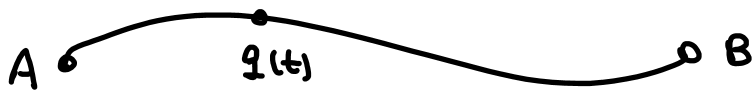
\includegraphics[width=0.35\textwidth]{question_action_newton}}
   \titem{
       \item 牛顿视角:已知初始位置和初始速率。在各个时刻,这个粒子“感觉”到了一个力并根据那个力“调整”它的速率。这个调整过的速率“告诉”那个粒子怎么继续走。
       \item 最小作用量原理:起始点和终点为定点。这个粒子需要基于极限作用量“找到”这两点之间的路径。
   }
   能体会到作用量更“奇怪”了吗?一个粒子可以很直接的根据力场调整自己的速率(牛顿视角)。但是一个粒子是无法计算的(在计算理论中很重要,因为它甚至可能不携带一点信息或复杂到甚至可以成为一个逻辑门)。那么一个粒子是怎么遵循最小作用量原理的呢?

   此外,我们之前还提出了最小作用量原理是一个解释自然法则的更基础的方式。那么为什么自然最基本的行为是如此“怪异”的呢?
}

\textbox{自然是自然的,但量子的\index{路径积分}}{
    不是。
    \marginnote{你可能会思考一个相似的问题:为什么在电路中,电流“知道”走哪条路来最小化功率?答案是不,电流是不知道的。其实是电场会建立所有可能的路径,直到达到一个稳定状态。一个更显然的例子是为什么一场洪水“知道”流到哪里。很显然,这些都是经典物理的问题。但是一个粒子需要依靠它的量子性质来达成相似的效果。}
    自然并不是怪异的。自然是很自然的,只不过不是经典物理的。
    
    让我们回到粒子运动的问题。与其“计算”极限作用力,粒子事实上“试了”\emph{每一种可行的路径}并“选择”了最极限的那个。

    \tcblower

    上面的话其实只是量子力学中的路径积分公式。在量子力学中,一件事发生的可能性$P$(这里:粒子从$A$传播到$B$)被分解为
    \begin{align}
        P = |\mathcal{A}|^2~,
    \end{align} 
    这里的复数$\mathcal{A}$被称为概率幅度。概率幅度可以通过所有路径的加权平均来计算
    \begin{align}
        \mathcal{A} \propto \sum_{\small \mbox{all paths}} e^{iS/\hbar} ~.
    \end{align}
    这里的“所有路径”表示了所有可能的联结$A$和$B$的线。它们不一定满足运动方程。
}

\mtextbox{如果$S\sim \hbar$呢?} {那$S \sim \hbar = 1.05\times 10^{-34}$ $\mbox{m}^2$kg/s时会怎样呢?让我们在下节走进了量子力学的新世界再来回答这个问题!事实上,我们会用一个不一样但是等效的量子力学的表示(主要是波力学与一些方阵力学)来代替路径积分。这是因为路径积分虽然概念很好理解,但是计算起来并不简单。在一个完整的量子力学的课程里会学到它。}
\textbox{作用量原理的说明\index{从量子到经典}}{
    在量子的世界里,作用量的物理意义很明确--$e^{iS/\hbar}$是作为所有路径总和中路径的权重的相位因子。
    
    你可能会困惑为什么在经典力学中,粒子只会选择一个路径。在量子力学中(路径积分的表述):这个粒子沿着所有可能的路径移动。如何调和差异?经典路径如何出现在量子路径中?

    \tcblower

    当$S\gg \hbar$时,经典力学从量子力学中出现了。在这个限制下,即使$S$的微小变化(由于选择附近不同的路径)也会导致单位$\hbar$ 发生很大变化,因此$e^{iS/\hbar}$是一个快速的振荡函数,它消除了几乎所有不同路径的贡献。

    不过只有一个例外:接近固定作用量$\delta S=0$时。接近$\delta S=0$的不同路径不会消掉。因此经典路径在取经典极限$S\gg \hbar$时,是唯一剩下的路径。
}

\section{结语:总结和下一步}

\textbox{额外参考阅读}{
    \titem{
        \item 其他教科书中的类似内容:你可以在泽的\href{https://www.amazon.com/Einstein-Gravity-Nutshell-Zee/dp/069114558X}{《爱因斯坦引力论概论》}第二部分找到对这里内容更深的讨论。你也可以阅读鲍曼的\href{http://www.damtp.cam.ac.uk/user/db275/concepts/Concepts.pdf}{现代物理学的讲义}的第一节和附录。
        \item 如果你需要更多的参考,我推荐观看苏斯金德的\href{http://theoreticalminimum.com/}{理论最小量(视频讲座)}  (经典力学的讲座3和4)。或者阅读戈尔茨坦、小普尔和萨夫科写的\href{https://www.amazon.com/Classical-Mechanics-3rd-Herbert-Goldstein/dp/0201657023}{《经典力学》}的第二章。 
    }
}

\textbox{在大学物理系中还会学什么?}{
    \titem{
        \item 经典力学:最小作用量与经典力学中的拉格朗日公式是紧密相连的。还有一个汉密尔顿公式。你会学到如何用这些方式来描述力学。你还会学到拉格朗日力学对求解限制运动的问题是有什么样的帮助。
        \item 量子力学:这里提到的路径积分会是量子力学(有时候也叫做进阶量子力学)的一部分。(量化的)汉密尔顿量也是量子力学很核心的一部分。
        \item 量子场论:一个量子场论的模型是从一个作用量开始的。你会在那里看到最小作用量原理是作为第一定律。
    }
}

\section{练习}

\textbox{练习1.1 费马原理的折射}{
    推导费马原理中的折射定律。
}

\textbox{练习1.2 极限但非最短路径}{
    找一个光沿极限但不是最短的路径走的例子。
}

\textbox{练习2.1 一个宇宙的标量场}{
    在宇宙学中,一个均匀且相同的标量场有作用量
    \begin{equation}
    S = \int dt ~ a^3(t) \left(
        \frac{1}{2}\dot\phi^2 - V(\phi)
    \right)~, \nonumber
    \end{equation}
    $a(t)$是一个时间的函数。$V(\phi)$是$\phi$的函数。
    用两种方式(欧拉-拉格朗日方程和变换原理)明确的计算$\phi$的欧拉-拉格朗日方程(即$\ddot\phi$、$\dot\phi$和$\phi$之间的关系)。
}

\textbox{练习3.1 从欧拉-拉格朗日到牛顿}{从欧拉-拉格朗日方程开始,用一个牛顿力学中的粒子的拉格朗日量推导出势能中粒子运动的牛顿第二定律。}

\textbox{练习3.2 相对论性自由粒子\index{相对论性自由粒子的作用量}}{
    一个相对论性自由移动的粒子(即并非在力场中或与其他粒子有相互总用)的作用量是
    \begin{align}
        S = \alpha \int d\tau = \alpha \int \sqrt{1-\frac{\dot q^2}{c^2}} ~ dt ~,
    \end{align}
    $\alpha$为常数。
    \titem{
        \item 运用牛顿极限$\dot q \ll c$求$\alpha$的值。
        \item 证明这个系统具有时间平移对称性。
        \item 推导相对论能量是时间平移的守恒量。
    }
}

\printindex

\end{document} 